\section{Building Trusted Path with \name}
\label{sec:secureInput}

%\iffalse
%\begin{figure}[t]
% \centering
%  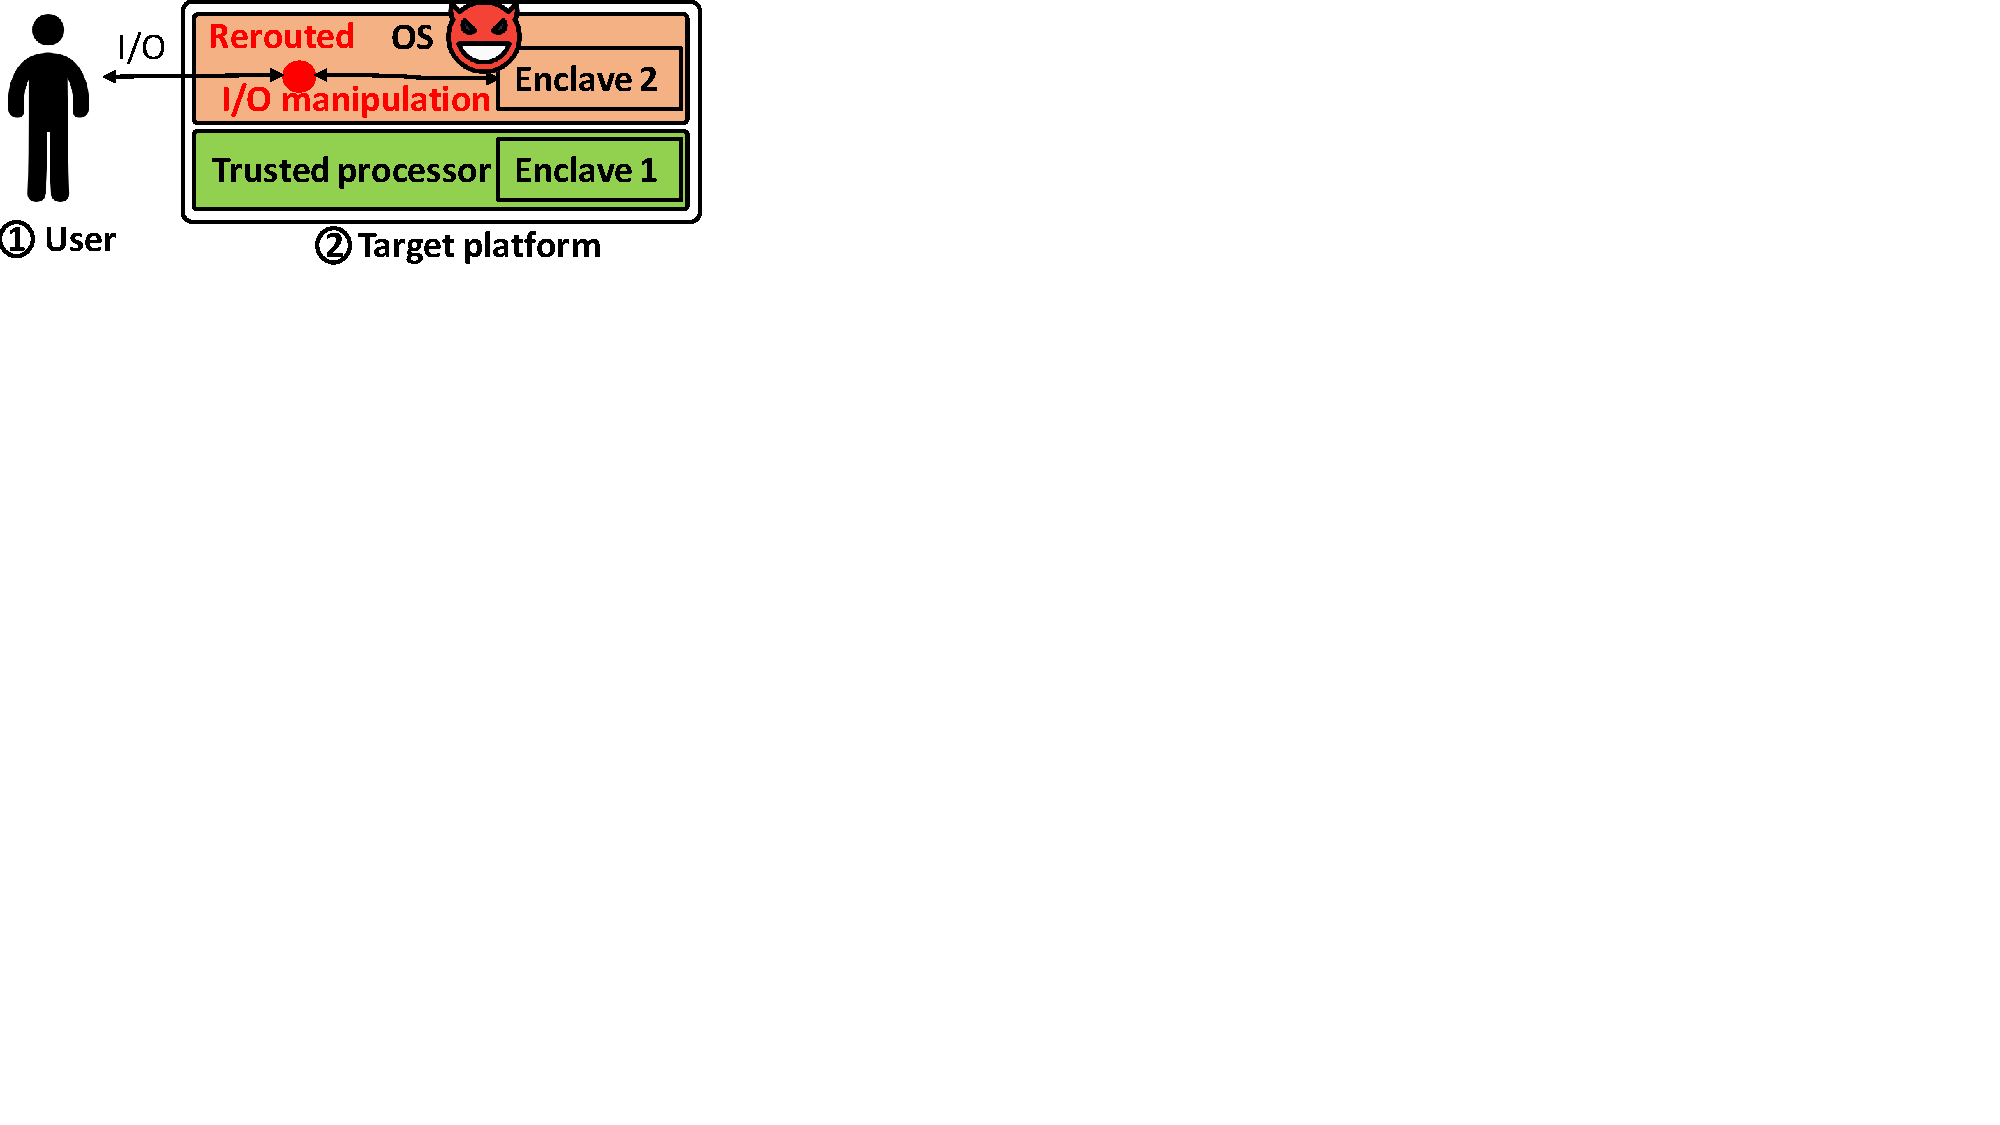
\includegraphics[trim={-1cm 14.5cm 19cm 0},clip,width=0.6\linewidth]{EnclaveSwitchAttack_revised.pdf}
% \caption{\textbf{Trusted path model and attacks.} The OS can see and manipulate all the I/O operations done by the user. Additionally, the attacker can reroute user input to another enclave than the user intended.%\vspace{-25px}
% }
% \label{fig:enclaveSwitching}
%\end{figure}
%\fi

One important limitation of SGX is the lack of \emph{trusted path}. As defined in~\cite{filyanov2011uni}, a trusted path (i) isolates the input and output channels of different applications to preserve the integrity and confidentiality of data exchanged with the user, (ii) assures the user of a computer system that she is truly interacting with the intended software, and (iii) assures the running applications that user inputs truly originate from the actions of a human, as opposed to being injected by other software.

%As shown in Figure~\ref{fig:enclaveSwitching}, 
In SGX, an attacker who controls the OS can trivially read and modify all user's inputs, read and modify all enclave's outputs intended to the user, and direct the user's inputs to a different enclave from the one intended by the user. Under the SGX security model, the lack of a trusted path prevents the user from providing sensitive information like passwords to enclaves or confirming transactions performed by the enclave.



The commonly suggested solution for the trusted path problem is to leverage a trusted hypervisor to mediate all I/O~\cite{weiser2017sgxio}. The main drawback of general-purpose (commercial) hypervisors is their significant complexity and attack surface. While the research community has also produced small and formally-verified hypervisors, like the seL4 project~\cite{klein2009sel4}, their adoption in practice can be problematic. In addition to the secure hypervisor itself, a realization of a trusted path requires secure device drivers, which can be difficult to implement and increase the TCB size. Formally-verified hypervisors are also typically severely restricted in terms of functionality, and adding new functionality to it and can be very slow, as each new update needs to be formally verified (a process that can take years). For these reasons, minimal and formally verified hypervisors are not commonly used in consumer devices or corporate systems that require rich functionality and updates.

\begin{figure}[t]
 \centering
 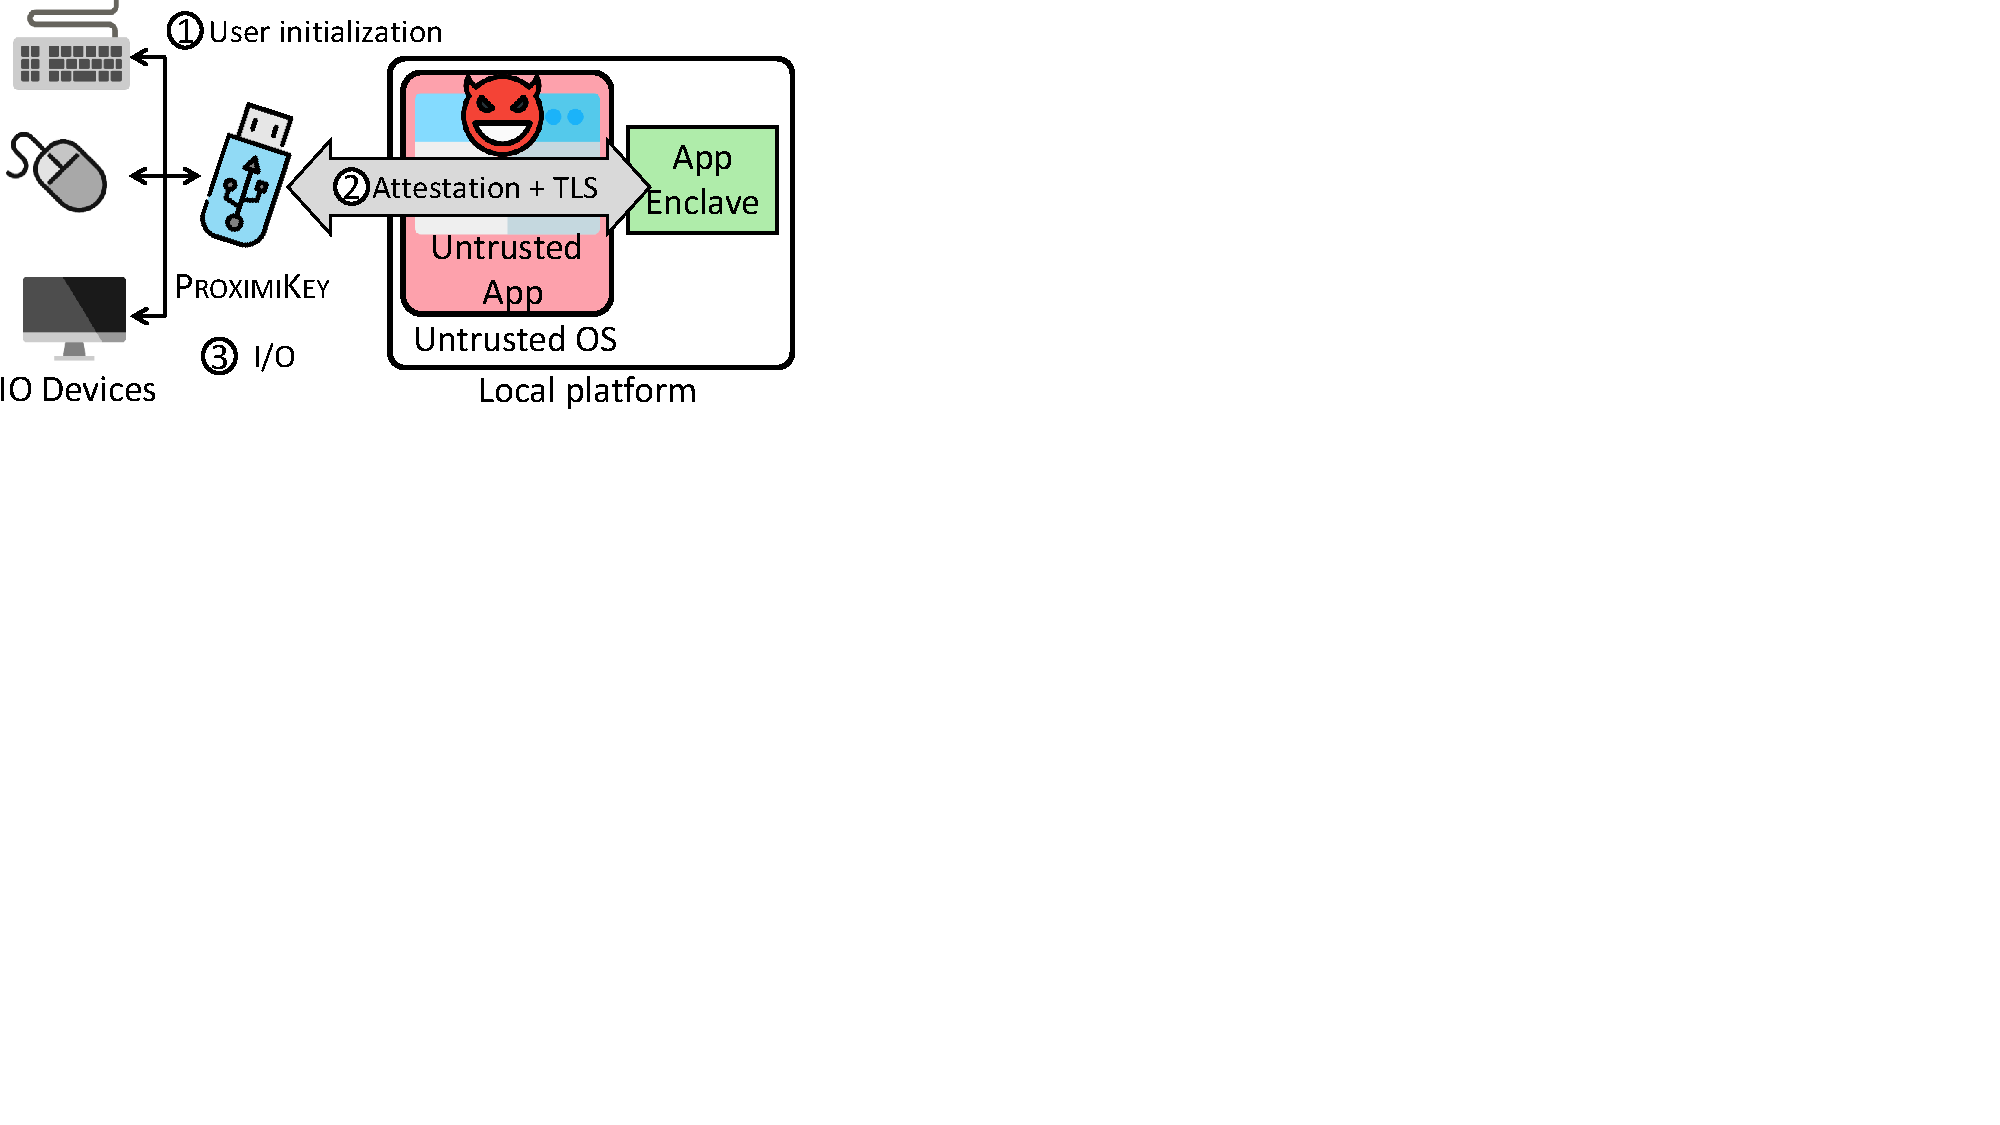
\includegraphics[trim={0 12cm 20cm 0},clip,width=0.65\linewidth]{chapters/ProximiTEE/images_new/trustedPath.pdf}
 \caption[Trusted path to local enclave using \device]{\textbf{Trusted path to local enclave using \device.} The IO devices are connected to \device that is connected to the local platform. The \device performs attestation using one of our mechanisms and then mediates all IO communication.}

 \label{fig:secureInput}
\end{figure}

\subsection{Our approach}

In this section, we explain how our attestation mechanisms can be used to build a trusted path between the user and an enclave. Our main idea is to use the \device device as a \emph{bridge} that attests the local enclave and then securely mediates all user inputs and outputs between I/O devices and enclaves, as shown in Figure~\ref{fig:secureInput}. A trusted path can be realized using either of our two attestation mechanisms as a building block.

For trusted path, we require that the \device device has at least two communication interfaces, one for the target platform and additional ones for the I/O device(s), and minimal user interaction capabilities, e.g., a small display and a button. We also assume that the embedded device is either (i) pre-installed with a list of human-readable names for enclave code measurements, or (ii) it can obtain certified mappings from the platform that it is connected to, similar to property-based attestation~\cite{SadeghiProperty}.

We assume that the user activates the trusted path by selecting the enclave with which she wishes to communicate using a button on the device, and the enclave name is shown on the device screen.%\footnote{Alternatively, the interaction can be initiated by an untrusted application or the OS. In this case, the embedded device can show the human-readable enclave name on its screen that the user can verify.} 

%We discuss the benefits and drawbacks of these two known approaches in Section~\ref{sec:discussion}.



\subsection{Local trusted path} 

Now, we describe the process of establishing a trusted path to an enclave on a \emph{local} platform. As shown in Figure~\ref{fig:secureInput}, the I/O devices are connected to the \device that is attached to a local computing platform. The trusted path creation proceeds as follows:

\begin{enumerate}
    \item[\one] The user selects which enclave to use using a button and a display on \device.
    \item[\two] \device performs attestation of the chosen enclave using either of our two attestation mechanisms. \device verifies that the measurement of the attested enclave matches the user's selection. \device establishes a secure channel (TLS) to the correct enclave.
    \item[\three] \device captures all the input from the I/O devices and sends them to the enclave via the secure channel. Similarly, the enclave can send output to the user over the same channel.
\end{enumerate}
 

\begin{figure}[t]
 \centering
  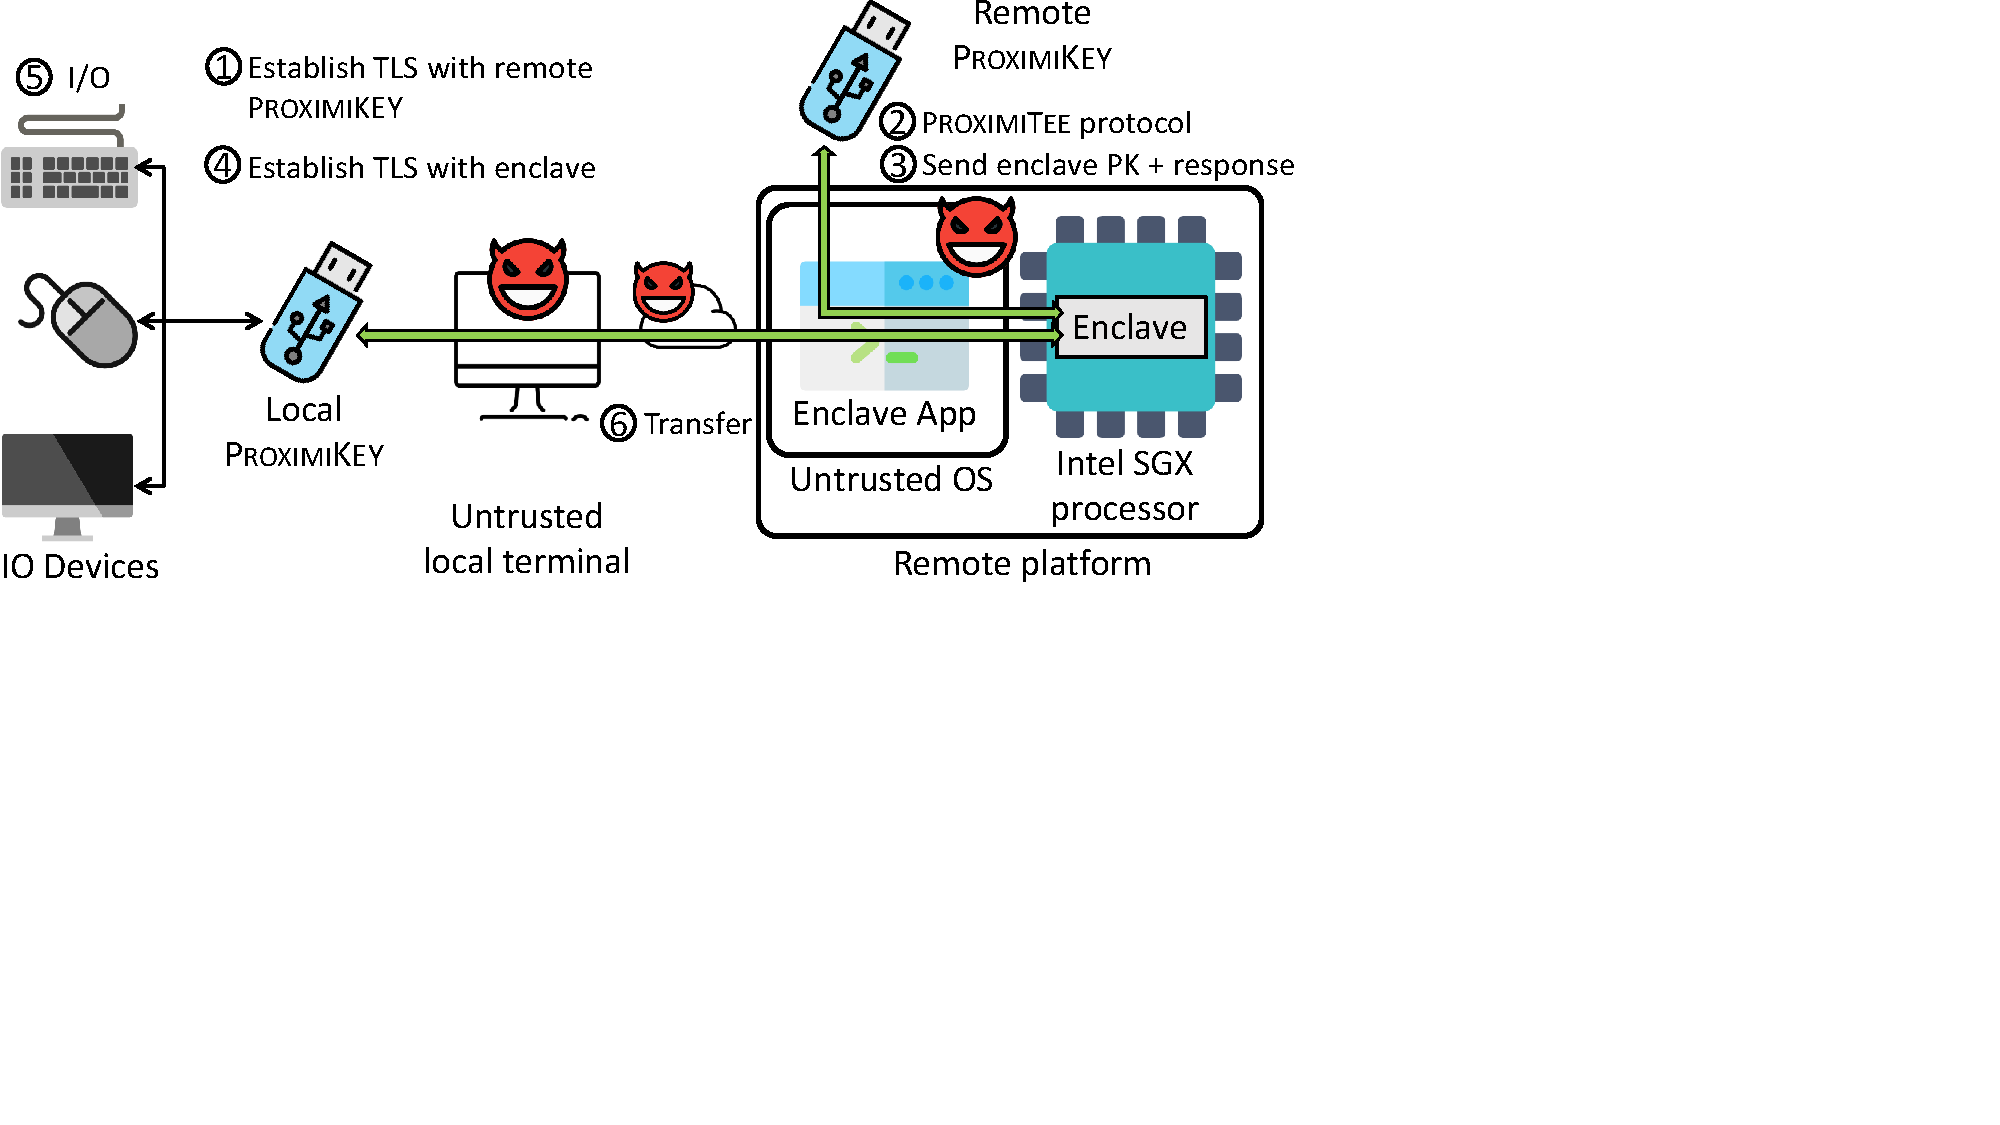
\includegraphics[trim={0 8cm 12cm 0},clip,width=0.85\linewidth]{chapters/ProximiTEE/images_new/SystemDesignRemote.pdf}
 \caption[Trusted path to a remote enclave using \device]{\textbf{Trusted path to a remote enclave using \device.} This setup uses two embedded devices. The local \device is connected to the local platform and the remote \device is connected with the remote platform.}
 \label{fig:systemRemoteHost}
\end{figure}

\subsection{Trusted Path to a Remote Enclave} 

Next, we describe how such a trusted path can be extended to an enclave that resides on a \emph{remote platform}, as shown in Figure~\ref{fig:systemRemoteHost}. Both the local and the remote platforms have a \device device attached to them. The I/O devices are attached to the local \device. Trusted path creation proceeds as follows:

\begin{enumerate}
	\item[\one] The user initiates the trusted path by selecting an enclave as explained above.
	\item[\two] The local \device acts as the remote verifier in remote attestation using one of our attestation mechanisms. As the end result of the attestation process, the local \device has established a secure channel to the correct enclave via the remote \device.
	\item[\three] The user can securely communicate with the enclave.
\end{enumerate}

 
\begin{figure}[t]
  \centering
    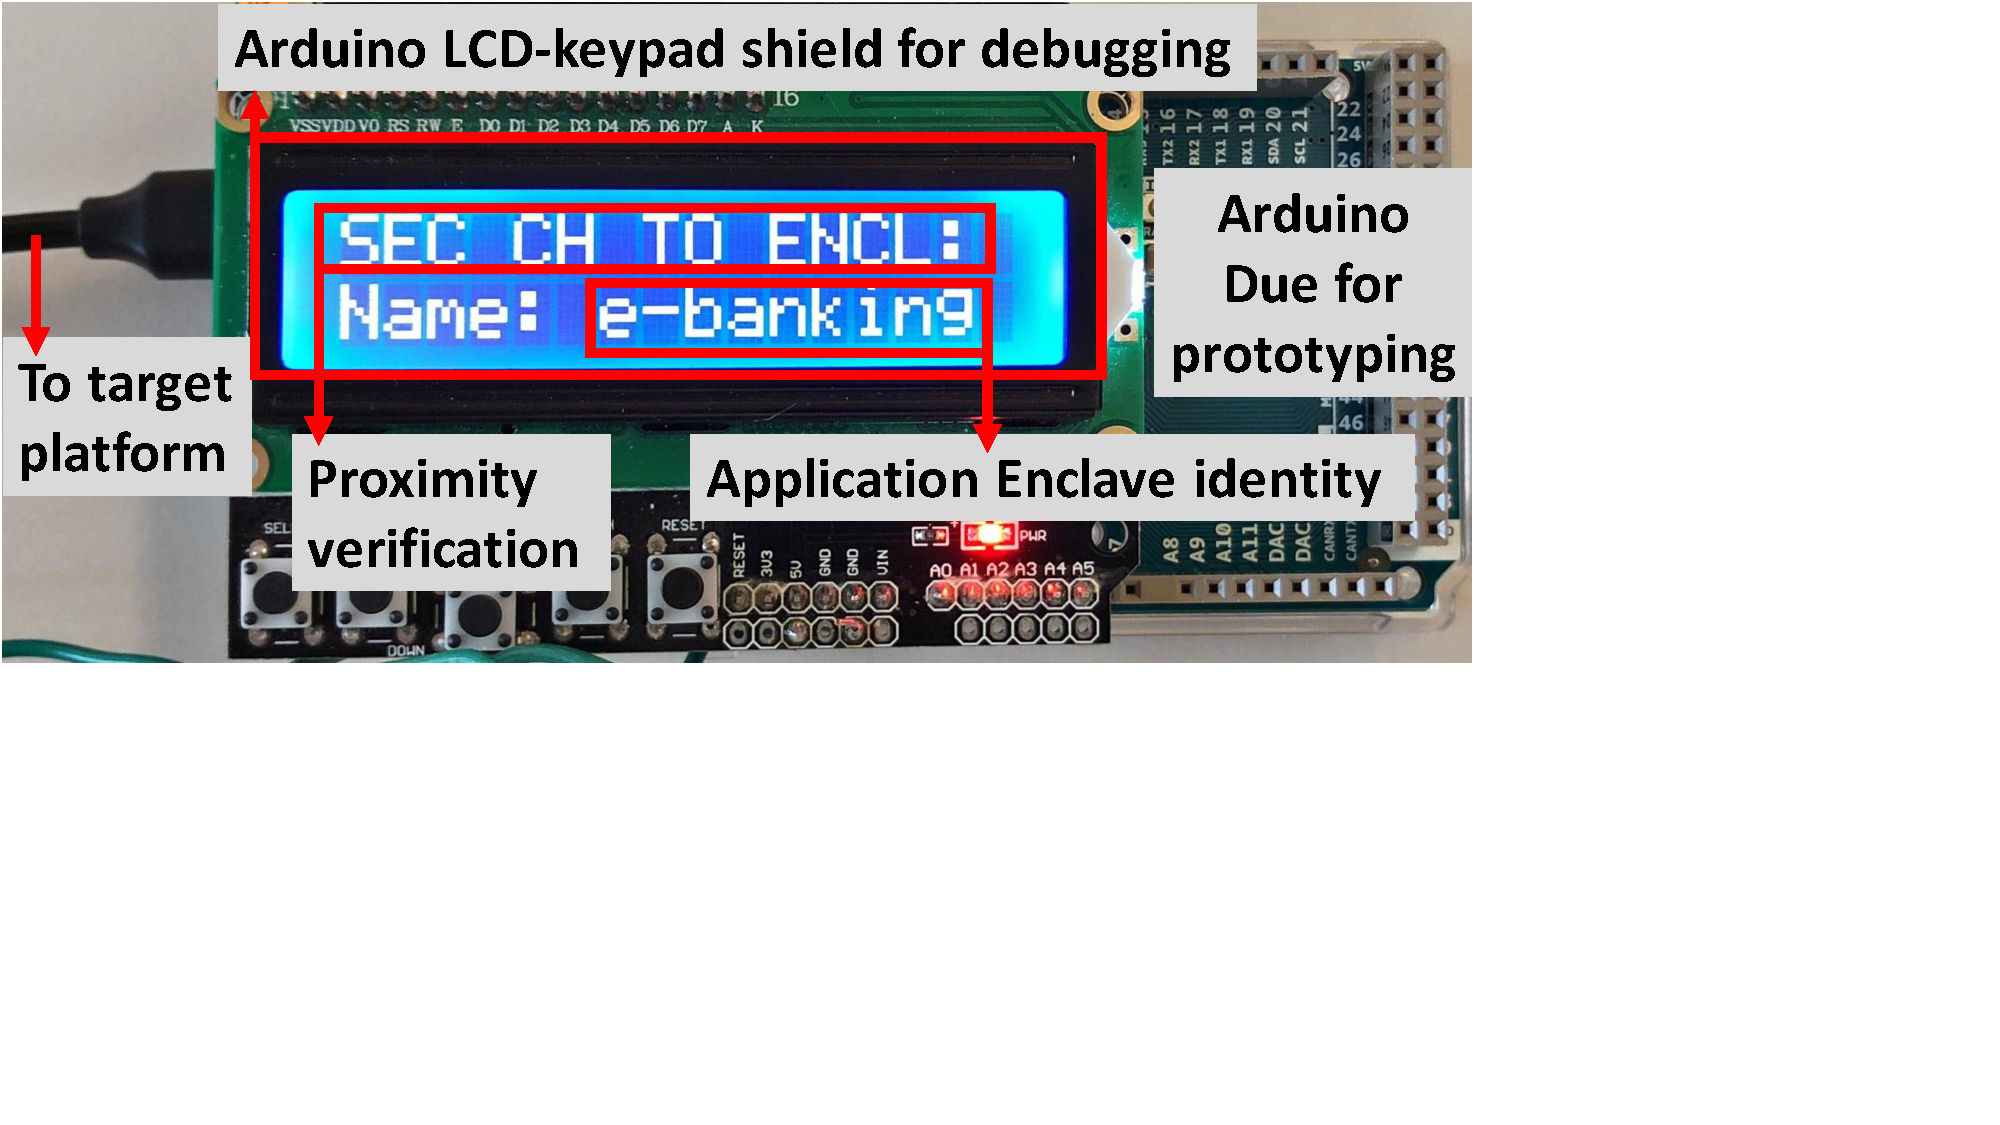
\includegraphics[trim={0 7.5cm 9cm 0}, clip, width=0.7\linewidth]{chapters/ProximiTEE/images/Setup1.pdf}
    \caption[\name trusted path implementation]{\textbf{\name trusted path implementation.} The figure shows the \device based on Arduino Due prototype board that is used as an I/O hub for trusted path implementation. The \device also uses a small LCD display to show the identity of the SGX enclave that is is communicating with.}
    \label{fig:trustedPathImplementation}
\end{figure}


\myparagraph{Implementation} 
Figure~\ref{fig:trustedPathImplementation} shows our trusted path implementation that is based on an Arduino Due prototyping board. We implement a minimal prototype that handles keyboard communication using Ardubnio's native \texttt{keyboardcontroller} library that intercepts keyboard traffic. All the keystrokes are relayed to the application-specific enclave over the \tls channel. 
%
We additionally attach an LCD shield on the Arduino board that shows the enclave identity (name) with which it is currently communicating. This identity is obtained from a certificate that is embedded in the enclave.

%the application-specific enclave to aid the user to understand the identity of the enclave she is communicating with.


